\section{Approach}
Our goals were to create a modular framework that:
\begin{enumerate}
\item allows for extension by other developers, but without specific domain knowledge
\item provides for consistent parameterized simulation
\item allows for diverse simulations tailored to realistic SCADA conditions
\end{enumerate}
\subsection{Simulated Network}

\subsection{Controller}

\subsubsection{Actuator}

\subsubsection{Sensor}

\subsubsection{Internet Cloud}

\subsubsection{Factory Access Point}

\subsubsection{Factory Bridge}

\subsection{Matlab Simulation}

\subsubsection{Tennessee Eastman}

\subsection{C++ to Matlab Bridge}


\begin{figure*}
        \centering
		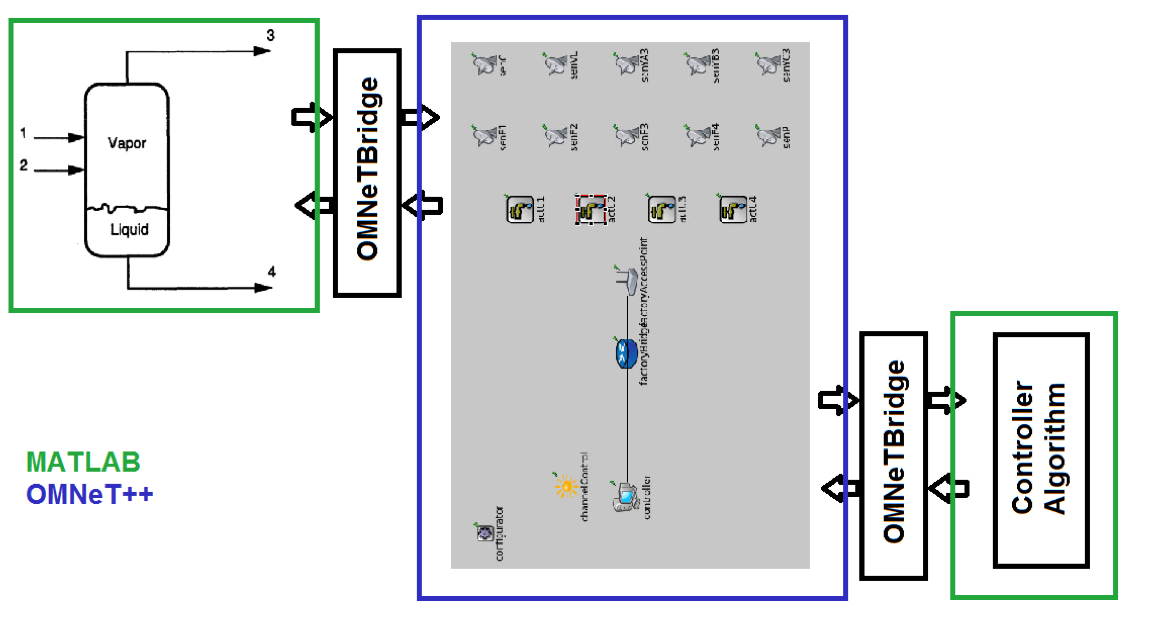
\includegraphics[width=0.8\textwidth]{figs/system.png}
        \caption{System Diagram.}
        \label{fig:system}        
\end{figure*}